\chapter{Testovanie}
\label{kapitola6}
V tejto kapitole sa nachádza popis a postup jednotlivých testov aplikácie, doplnený s obrázkami z testovacích prostredí. Pri testovaní sa použil nástroj Cypress a Postman. Práca s nimi je podrobnejšie popísaná nižšie.  

\section{Testovanie medzi dvomi stranami(End-to-End)}
Testovanie medzi dvomi stranami, alebo End-to-End testovanie slúži na testovanie funkcionality celej aplikácie. Na rozdiel od jednotkových testov, ktoré testujú iba časť kódu, end-to-end testy prechádzajú celú aplikáciu z pohľadu užívateľa. Tieto testy sú dôležitou súčasťou aplikácie, umožňujú odchytenie chýb pri zmenách v zdrojovom kóde a zaručujú očakávané správanie od začiatku až do konca.

\subsection{Cypress}
Cypress je nástroj pre webové aplikácie, ktorý umožňuje vytváranie testov medzi dvomi stranami. Nástroj ponúka širokú škálu funkcionalít, pomocou ktorých sa dá otestovať každý jeden element webovej stránky. Cypress prechádza celú aplikáciu, simuluje správanie užívateľa. Umožňuje klikanie na tlačítka, písanie do políčok, alebo aj presmerovanie na inú URL adresu. Poskytuje prehľadné užívateľské rozhranie, kde simuluje užívateľom vybraný prehliadač. Jednotlivé testy sa dajú spustiť naraz, ale aj zvlášť po častiach. Po vytvorení účtu a prihlásení, cypress uchováva históriu testov, ku ktorým sa dá hocikedy vrátiť. Nástroj umožňuje náhľad do testu v priebehu testovania, kde je vidieť každý jeden krok testu, s ktorými elementami sa pracovalo a aké akcie sa vykonali. K jednotlivým krokom sa v ktoromkoľvek okamihu počas testovania dá vrátiť.

Cypress sa inštaluje klasicky ako každý iný balík cez správcu balíčkov npm a spúšťa sa cez príkaz v termináli \texttt{npx cypress open}. Po prvom spustení sa v hlavnom adresári klienta vytvorí zložka \texttt{cypress}, s ktorou sa ďalej pracuje. Jednotlivé testy sa nachádzajú v zložke \texttt{cypress/integration}. End-to-End testy v aplikácii sú rozdelené na dve hlavné časti, \texttt{auth} a \texttt{presentation}. K jednotlivým elementom používaným v testoch sa pristupuje cez HTML data atribút. Tieto elementy sú v šablóne označené cez atribút \texttt{data-test}, napríklad: \texttt{<b-input data-test="email" />}. Pri ich potrebe sa element vyhľadá a zvolí pomocou cypress funkcie a vykoná sa potrebná akcia nad ním.

Po úspešnom priebehu, cypress označí test zelenou fajkou a pri narazení na chybu červeným krížom. Po dokončení testovanie sa zobrazí súhrn testovania a čas v sekundách trvania celého testu viď. obrázok \ref{pic:cypress}.

    \begin{figure}[!hbt]
        \centering
        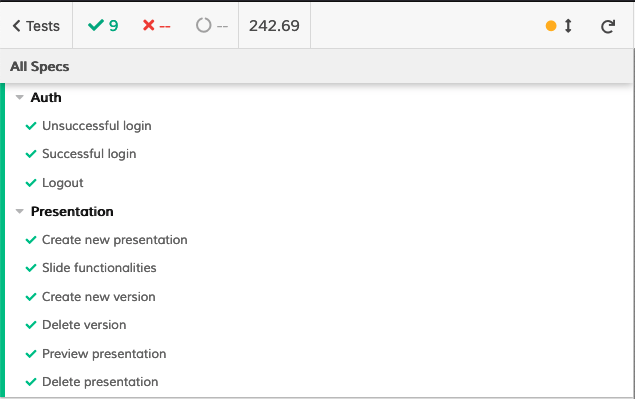
\includegraphics[scale=0.4]{obrazky/cypress.png}
        \caption{Súhrn dokončeného testovania}
        \label{pic:cypress}
    \end{figure}

\subsection*{Autentifikačné testy}
Autentifikačné testy sa nachádzajú v súbore \texttt{cypress/integration/auth.ts}. Tento súbor obsahuje testy:

    \begin{itemize}
        \item\textbf{Unsuccessful Login} - testuje sa zobrazenie chybovej hlášky pri neúspešnom prihlásení cez tlačítko.    
        \item\textbf{Successful Login} - testuje sa vyplnenie správnych prihlasovacích údajov a prihlásenie cez tlačítko.
        \item\textbf{Logout} - testuje sa odhlásenie cez tlačítko a presmerovanie na stránku prihlásenia.
    \end{itemize}
    
\subsection*{Testy prezentácie}
V súbore \texttt{cypress/integration/presentation.ts} sa nachádzajú všetky testy týkajúce sa prezentácií, od ich tvorby až k odstráneniu. Tento súbor obsahuje testy:

    \begin{itemize}
        \item\textbf{Create new presentation} - v tomto teste sa kontroluje, že daný užívateľ najprv nemá žiadne vytvorené prezentácie. Prezentácia sa vytvorí cez tlačítko. \texttt{CREATE NEW} a otestuje sa, či URL adresa odpovedá adrese \texttt{/presentation/new} a či je editor viditeľný. Cez tlačítko sa otvorí panel pre uloženie prezentácie a následne sa vyplnia potrebné údaje pre uloženie. Pomocou tlačítka sa vráti na domovskú stránku, kde sa skontroluje či zoznam obsahuje uloženú prezentáciu.
        
        \item\textbf{Slide functionalities} - v tomto teste sa kontrolujú všetko funkcionality nad stránkami prezentácie. Najprv sa otvorí prezentácia v editore cez tlačítko na domovskej stránke. Cez tlačítko sa otvorí bočný panel obsahujúci stránky prezentácie. Prezentácia v tomto okamihu obsahuje iba jednu stránku. Otestuje sa, že pri jednej stránke je tlačítko odstránenia stránky nefunkčné. Nasleduje test kopírovania a vloženia stránky. Otestuje sa pridanie novej stránky cez tlačítko a jeho odstránenie. V poslednom kroku sa kontroluje mriežkový pohľad stránok.
        
        \item\textbf{Create new version} - v tomto teste sa pracuje s verziami prezentácie. Znova sa prezentácia otvorí v editore, kde sa uloží pod iným názvom ako verzia číslo 2. Na domovskej stránke sa otestuje, že zoznam stále obsahuje iba jednu prezentáciu, ale s iným názvom. Zobrazí sa detail prezentácie a skontroluje sa počet prezentácií. Otestujú sa rôzne popisy jednotlivých verzií. Otvorí sa verzia číslo 2 v editore a uloží sa pod iným názvom a rozličným popisom pod rovnakou verziou. Na domovskej stránke sa znova skontroluje počet prezentácií, počet verzií a či verzia číslo 2 obsahuje nové údaje. 
        
        \item\textbf{Delete version} - v tomto teste sa rieši odstránenie verzie prezentácie. Mazanie sa uskutoční cez tlačítko na domovskej stránke, aplikácia si vyžiada potvrdenie o mazaní. Po odstránení sa skontroluje počet verzií prezentácie.
        
        \item\textbf{Preview presentation} - v tomto teste sa testuje zobrazenie prezentácie v prezentačnom móde cez tlačítko na domovskej stránke. Kontroluje sa či URL adresa obsahuje text \texttt{/preview}.
        
        \item\textbf{Delete presentation} - test kontroluje úspešné odstránenie celej prezentácie cez tlačítko na domovskej stránke. Po odstránení sa testuje prázdny zoznam prezentácií. 
    \end{itemize}
    
\section{Testovanie aplikačného rozhrania}
Aplikačné rozhranie sa počas vývoja testovalo cez nástroj Postman. Postman je pomôcka, ktorá umožňuje zasielanie HTTP dotazov na koncové body a prijímanie odpovedí od nich. Nástroj poskytuje prehľadné užívateľské rozhranie, kde stačí zadať URL adresu koncového bodu. Užívateľské rozhranie obsahuje históriu poslaných dotazuv, ku ktorým sa dá kedykoľvek vrátiť. Postman taktiež umožňuj jednoduché pridávanie query parametrov, obsahu tela dotazu a upravovanie hlavičky dotazu. Odpoveď na dotaz je možné zobraziť vo viacerých formátoch. Prostredie nástroja je zobrazené na obrázku \ref{pic:postman}.

    \begin{figure}[!hbt]
        \centering
        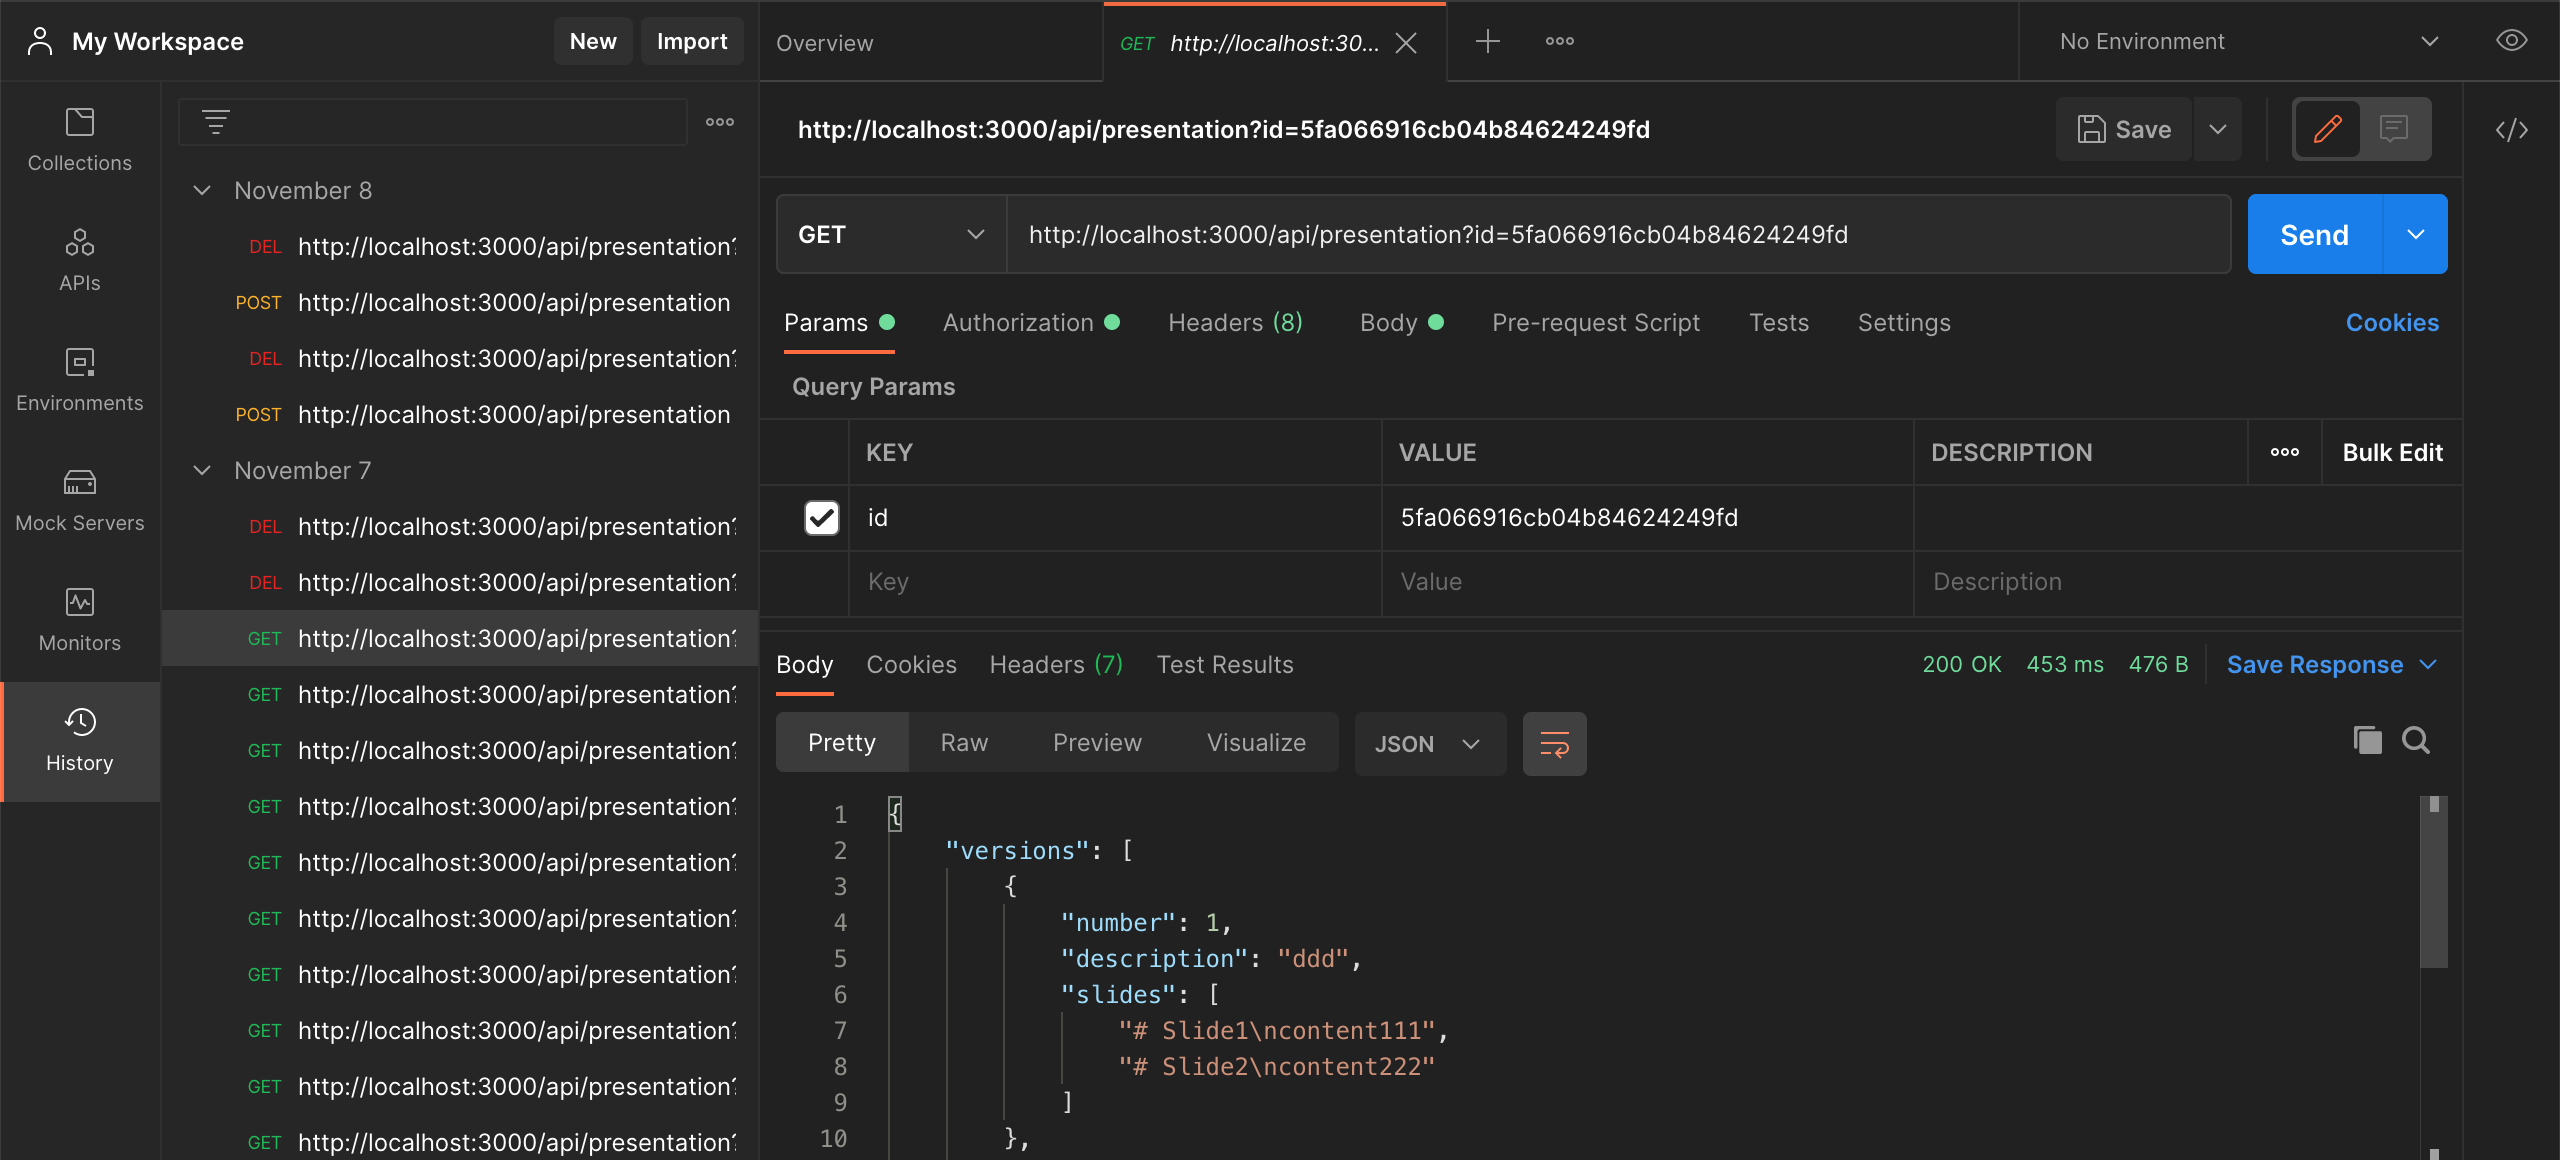
\includegraphics[scale=0.3]{obrazky/postman.png}
        \caption{Prostredie nástroja Postman}
        \label{pic:postman}
    \end{figure}